\documentclass{beamer}
\usepackage{listings}
\usepackage{mdframed}
\usepackage{tikz}
\usepackage{pdfpages}
\usepackage[francais]{babel}
\usepackage[utf8]{inputenc}
\usepackage{float}
\usepackage{graphicx}
\usepackage{wrapfig}
\usepackage{times}
\usepackage[T1]{fontenc}
\usepackage[overlay,absolute]{textpos}

\newcommand{\firstlogo}{mdl.png}
\newcommand{\secondlogo}{ups.jpg}
\newcommand{\footsubject}{Réponse à l'appel d'offre de la région PACA} 
\newcommand{\rgbcolortheme}{65,81,87}

\makeatletter
\hypersetup{pdfpagemode=FullScreen}

\mode<presentation> {
	\usepackage{../beamer-theme/beamerthemeUNLTheme}
}

\title[] % (facultatif, \`a utiliser uniquement si le titre de l'article est trop long)
{Réponse à l'appel d'offre de la région PACA}
\subtitle {TMA de l'application \bsc{Correlyce}}

\newcommand{\authors}{%
Julian \bsc{Bironneau}\newline
Antoine de \bsc{Roquemaurel}\newline 
Steve \bsc{Magras}\newline
Dylan \bsc{Roletto}\newline
Zaccaria \bsc{Zyat}\newline
}
\newcommand{\JulianSpeak}{%
\author[
\vspace{-30px}
\textbf{\color{white}J}ulian\\
Antoine\\
Steve\\
Dylan\\
Zaccaria
]{\authors}
}

\newcommand{\NooneSpeak}{
\author[
\vspace{-30px}
Julian\\
Antoine\\
Steve\\
Dylan\\
Zaccaria
]{\authors}
}

\newcommand{\AntoineSpeak}{
\author[
\vspace{-30px}
Julian\\
\textbf{\color{white}A}ntoine\\
Steve\\
Dylan\\
Zaccaria
]{\authors}
}

\newcommand{\SteveSpeak}{
\author[
\vspace{-30px}
Julian\\
Antoine\\
\textbf{\color{white}S}teve\\
Dylan\\
Zaccaria
]{\authors}
}
\newcommand{\DylanSpeak}{
\author[
\vspace{-30px}
Julian\\
Antoine\\
Steve\\
\textbf{\color{white}D}ylan\\
Zaccaria
]{\authors}
}
\newcommand{\ZacSpeak}{
\author[
\vspace{-30px}
Julian\\
Antoine\\
Steve\\
Dylan\\
\textbf{\color{white}Z}accaria
]{\authors}
}


\institute[] 
{
Universit\'e Toulouse III -- Paul Sabatier \\
M2 Informatique -- Développement Logiciel 
\vspace{-10px}
}

\date[ ~ ~ ~ 27 / 11 / 2015] % (facultatif, peut être une abr\'eviation du nom de la conf\'erence)
{Vendredi 27 Novembre 2015}



\AtBeginSection[] {
\begin{frame}<beamer>{Plan}
	\tableofcontents[currentsection,subsectionstyle=hide]
\end{frame}
}

%\setbeamerfont*{section in sidebar}{size=\fontsize{6px}{2.3em}\selectfont }
%\setbeamerfont*{subsection in sidebar}{size=\fontsize{5px}{1.5em}\selectfont }
\begin{document}
	\sidetoc{no}
	\NooneSpeak{}
	\begin{frame}
		\titlepage
	\end{frame}

	\sidetoc{yes}
	\AntoineSpeak
	\begin{frame}
		\tableofcontents[subsectionstyle=hide]
	\end{frame}
		\AntoineSpeak
	\section{Présentation générale} % Intro + Projet &=&  4'
	\subsection{La société GlobalSoftTech}
	\begin{frame}{La société GlobalSoftTech}
		\begin{itemize}
			\item SSI spécialisée développement Web
			\item Taille moyenne
			\item Chiffre d'affaire de 100 millions d'euros
			\item + de 200 clients dans le monde
			\item Expérience dans la TMA
		\end{itemize}
	\end{frame}

	\section{Offre technique générale} %  Méthodo = 8'
	\subsection{Enjeux}
\JulianSpeak
\begin{frame}{Enjeux}
\begin{itemize}
	\item Confirmer la position
	\begin{itemize}
		\item Améliorer son taux d'utilisation
		\item Étendre sa visibilité
		\item Faire de \bsc{Correlyce} une référence
	\end{itemize}
	\vfill
	\pause
	\item Logiciel libre
		\begin{itemize}
			\item Conserver la licence GPL
			\item S'inscrire dans la stratégie de région PACA
		\end{itemize}
			\vfill
	\pause			
	\item Expérience en agilité
\end{itemize}
\end{frame}
\subsection{Méthodologies et démarches}
\begin{frame}{Méthodologies et démarches}
	\begin{itemize}
		\item Une approche agile adaptée : KANBAN
		\item Allier la flexibilité de l'agilité et la maîtrise du risque
	\end{itemize}
	\begin{figure}[H]
		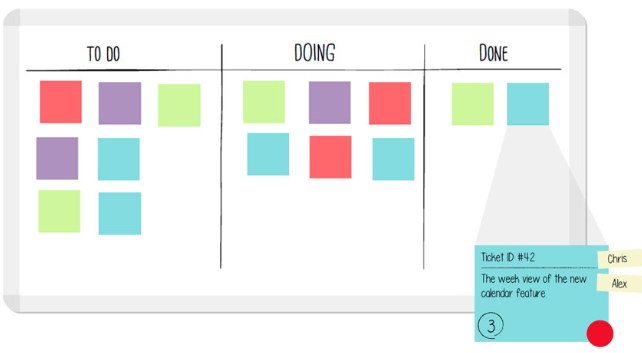
\includegraphics[width=8cm]{kanban.png}
		\caption{Fonctionnement du Board}
	\end{figure}
\end{frame}
\SteveSpeak
\subsection{Organisation de l'équipe}
\begin{frame}{Organisation de l'équipe}
		\begin{figure}[H]
			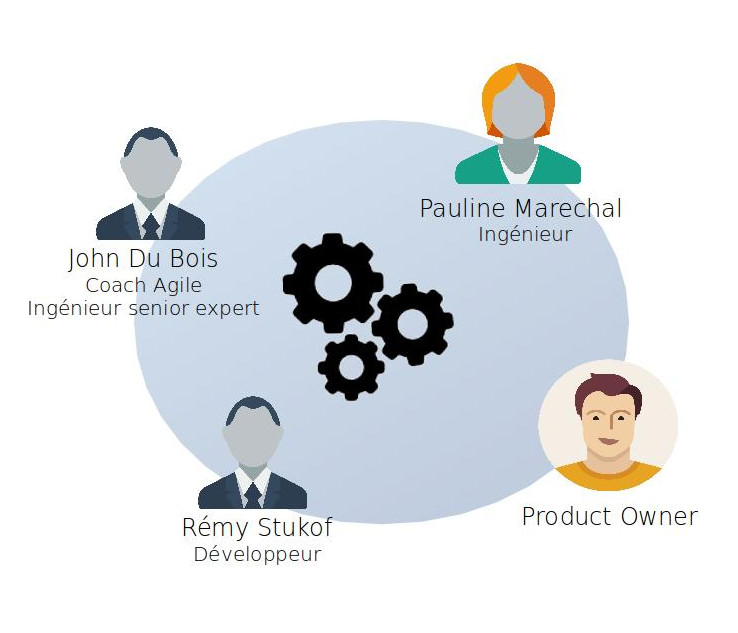
\includegraphics[width=8cm]{team.jpg}
			\caption{Organisation de l'équipe}
		\end{figure}
\end{frame}
\subsection{Moyens techniques}
\begin{frame}{Moyens techniques}
	\begin{itemize}
		\item Git et Github
		\item Travis CI
		\item Java (JUnit, CHeckStyle, PMD, Emma)
		\item SonarQube
		\item Heroku
		\item Zimbra
		\item Eclipse
	\end{itemize}
\end{frame}

	\section{Présentations des UO} % Résultats = 5'
	\ZacSpeak
\subsection{Étude et prestation de la TMA}
\begin{frame}{Étude et prestation de la TMA}
\end{frame}
\DylanSpeak
\subsection{Réversibilité}
\begin{frame}{Réversibilité}
\end{frame}
\AntoineSpeak
\subsection{Dispositif d'assistance}
\begin{frame}{Dispositif d'assistance}
\end{frame}
\DylanSpeak
\subsection{Prestation journalière à profil}
\begin{frame}{Prestation journalière à profil}
\end{frame}
\DylanSpeak
\subsection{Participation à la définition d'une gouvernance logicielle}
\begin{frame}{Participation à la définition d'une gouvernance logicielle}
\end{frame}

	\section{} % 3'
	\ZacSpeak
\begin{frame}{Conclusion}
	\begin{itemize}
		\item Une équipe professionnelle et compétente
		\item Une réalisation, un accompagnement et une réactivité de premier ordre
		\item Des tarifs ajustés
	\end{itemize}
	TODO tarifs
\end{frame}


	% Slide for questions
	\sidetoc{no}
	\NooneSpeak{}
	\begin{frame}{Avez-vous des questions ?}
		\begin{figure}[H]
			\centering
			
\includegraphics[width=5cm]{images/interrogation.png}
		\end{figure}
	\end{frame}
%	\vspace*{-7mm}    
%	\begin{frame}[plain]{Product Backlog}
%		\hspace*{-35mm}
%	%	\includegraphics[width=13.8cm]{backlog.pdf}
%	\end{frame}
%	\begin{frame}
%		\titlepage
%	\end{frame}
\end{document}
